
%{{第九回}}{第九回}}

\chapter{恋风流情友入家塾\\起嫌疑顽童闹学堂}

{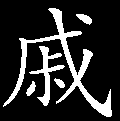
\includegraphics[width=3mm]{../Images/00005}\kaishu 君子爱人以道,不能减牵恋之情;小人图谋以霸,何可逃侮慢之辱?幻境幻情,又造出一番晓妆新样。}

话说秦业父子专候贾家的人来送上学择日之信。原来宝玉急于要和秦钟相遇,{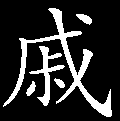
\includegraphics[width=3mm]{../Images/00005}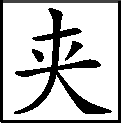
\includegraphics[width=3mm]{../Images/00012}\footnotesize \kaishu 妙!不知是怎样相遇。}却顾不得别的,遂择了后日一定上学。``后日一早,请秦相公先到我这里,会齐了,一同前去。''------打发人送了信。

至是日一早,宝玉起来时,袭人早已把书笔文物包好,收拾得停停妥妥,坐在床沿上发闷。{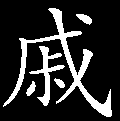
\includegraphics[width=3mm]{../Images/00005}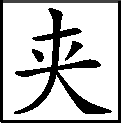
\includegraphics[width=3mm]{../Images/00012}\footnotesize \kaishu 神理可思,忽又写小儿学堂中一篇文字,亦别书中之未有。 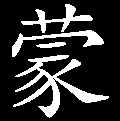
\includegraphics[width=3mm]{../Images/00006}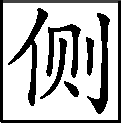
\includegraphics[width=3mm]{../Images/00011}\footnotesize \kaishu 此等神理,方是此书的正文。}见宝玉醒来,只得伏侍他梳洗。宝玉见他闷闷的,因笑问道:``好姐姐,{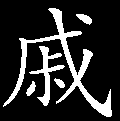
\includegraphics[width=3mm]{../Images/00005}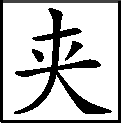
\includegraphics[width=3mm]{../Images/00012}\footnotesize \kaishu 开口断不可少此三字。}你怎么又不自在了?难道怪我上学去丢的你们冷清了不成?''袭人笑道:``这是那里话。读书是极好的事,不然就潦倒一辈子,终久怎么样呢。但只一件,只是念书的时节想着书,{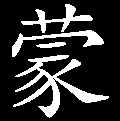
\includegraphics[width=3mm]{../Images/00006}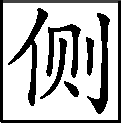
\includegraphics[width=3mm]{../Images/00011}\footnotesize \kaishu 袭人方才的闷闷,此时的正论,请教诸公,设身处地,亦必是如此方是,真是曲尽情理,一字也不可少者。}不念的时节想着家些。别和他们一处玩闹,{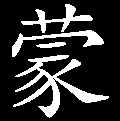
\includegraphics[width=3mm]{../Images/00006}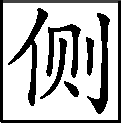
\includegraphics[width=3mm]{../Images/00011}\footnotesize \kaishu 长亭之嘱,不过如是。}碰见老爷不是玩的。虽说是奋志要强,那功课宁可少些,一则贪多嚼不烂,二则身子也要保重。这就是我的意思,你可要体谅。''{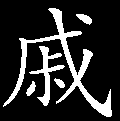
\includegraphics[width=3mm]{../Images/00005}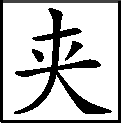
\includegraphics[width=3mm]{../Images/00012}\footnotesize \kaishu 书正语细嘱一番。盖袭卿心中,明知宝玉他并非真心奋志之人,袭人自别有说不出来之话。}袭人说一句,宝玉答应一句。袭人又道:``大毛衣服我也包好了,交出给小子们去了。学里冷,好歹想着添换,比不得家里有人照顾。脚炉手炉的炭也交出去了,你可逼着他们添。那一起懒贼,你不说,他们乐得不动,白冻坏了你。''宝玉道:``你放心,出外头我自己都会调停的。{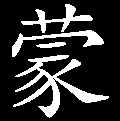
\includegraphics[width=3mm]{../Images/00006}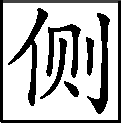
\includegraphics[width=3mm]{../Images/00011}\footnotesize \kaishu 无人体贴,自己扶持。}你们也别闷死在这屋里,长和林妹妹一处去顽笑才好。''说着,俱已穿戴齐备,袭人催他去见贾母、贾政、王夫人等。宝玉且又嘱咐了晴雯麝月等几句,{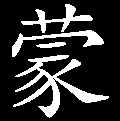
\includegraphics[width=3mm]{../Images/00006}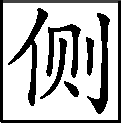
\includegraphics[width=3mm]{../Images/00011}\footnotesize \kaishu 这才是宝玉的本来面目。}方出来见贾母。贾母也未免有几句嘱咐的话。然后去见王夫人,又出来书房中见贾政。

偏生这日贾政回家早些,{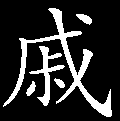
\includegraphics[width=3mm]{../Images/00005}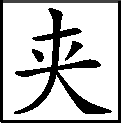
\includegraphics[width=3mm]{../Images/00012}\footnotesize \kaishu 若俗笔则又云不在家矣。试思若再不见,则成何文字哉?所谓不敢作安逸苟且塞责文字。}正在书房中与相公清客们闲谈。忽见宝玉进来请安,回说上学里去,贾政冷笑道:``你如果再提`上学'两个字,连我也羞死了。{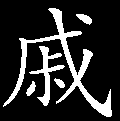
\includegraphics[width=3mm]{../Images/00005}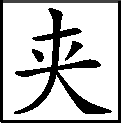
\includegraphics[width=3mm]{../Images/00012}\footnotesize \kaishu 这一句才补出已往许多文字。是严父之声。}依我的话,你竟顽你的去是正理。仔细站脏了我这地,靠脏了我的门!''{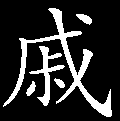
\includegraphics[width=3mm]{../Images/00005}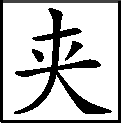
\includegraphics[width=3mm]{../Images/00012}\footnotesize \kaishu 画出宝玉的俯首挨壁之形象来。}众清客相公们都早起身笑道:``老世翁何必又如此。今日世兄一去,三二年就可显身成名的了,断不似往年仍作小儿之态了。天也将饭时,世兄竟快请罢。''说着便有两个年老的携了宝玉出去。

贾政因问:``跟宝玉的是谁?''只听外面答应了两声,早进来三四个大汉,打千儿请安。贾政看时,认得是宝玉的奶母之子,名唤李贵。因向他道:``你们成日家跟他上学,他到底念了些什么书!倒念了些流言混话在肚子里,学了些精致的淘气。等我闲一闲,先揭了你的皮,再和那不长进的算账!''{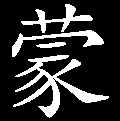
\includegraphics[width=3mm]{../Images/00006}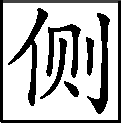
\includegraphics[width=3mm]{../Images/00011}\footnotesize \kaishu 此等话似觉无味无理,然而作父母的,到无可如何处,每多用此等法术,所谓百计经营、心力俱瘁者。}吓的李贵忙双膝跪下,摘了帽子,碰头有声,连连答应``是'',又回说:``哥儿已经念到第三本《诗经》,什么`呦呦鹿鸣,荷叶浮萍',小的不敢撒谎。''说的满座哄然大笑起来。贾政也撑不住笑了。因说道:``那怕再念三十本《诗经》,也都是掩耳偷铃,哄人而已。你去请学里太爷的安,就说我说了:什么《诗经》、古文,一概不用虚应故事,只是先把《四书》一气讲明背熟,是最要紧的。''李贵忙答应``是'',见贾政无话,方退出去。

此时宝玉独站在院外屏声静候,待他们出来,便忙忙的走了。李贵等一面弹衣服,一面说道:``哥儿可听见了不曾?先要揭我们的皮呢!人家的奴才跟主子赚些好体面,我们这等奴才白陪挨打受骂的。从此后也可怜见些才好。''{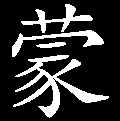
\includegraphics[width=3mm]{../Images/00006}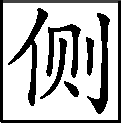
\includegraphics[width=3mm]{../Images/00011}\footnotesize \kaishu 可以谓能达主人之意,不辱君命。}宝玉笑道:``好哥哥,你别委曲,我明儿请你。''李贵道:``小祖宗,谁敢望你请?只求听一句半句话就有了。''说着,又至贾母这边,秦钟已早来候着了,贾母正和他说话儿呢。{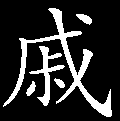
\includegraphics[width=3mm]{../Images/00005}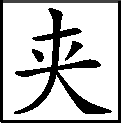
\includegraphics[width=3mm]{../Images/00012}\footnotesize \kaishu 此处便写贾母爱秦钟一如其孙,至后文方不突然。}于是二人见过,辞了贾母。宝玉忽想起未辞黛玉,{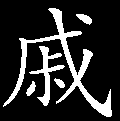
\includegraphics[width=3mm]{../Images/00005}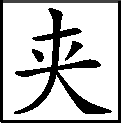
\includegraphics[width=3mm]{../Images/00012}\footnotesize \kaishu 妙极!何顿挫之至!余已忘却,至此心神一畅,一丝不漏。}因又忙至黛玉房中来作辞。彼时黛玉才在窗下对镜理妆,听宝玉说上学去,因笑道:``好!这一去,可定是要`蟾宫折桂'去了。{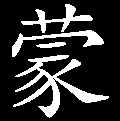
\includegraphics[width=3mm]{../Images/00006}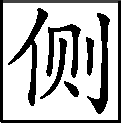
\includegraphics[width=3mm]{../Images/00011}\footnotesize \kaishu 此写黛玉,差强人意。《西厢》双文,能不抱愧!}我不能送你了。''宝玉道:``好妹妹,等我下学再吃晚饭。和胭脂膏子也等我来再制。''
唠叨了半日,方撤身去了。{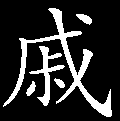
\includegraphics[width=3mm]{../Images/00005}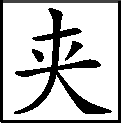
\includegraphics[width=3mm]{../Images/00012}\footnotesize \kaishu 如此总一句,更妙!}黛玉忙又叫住问道:``你怎么不去辞辞你宝姐姐来?''{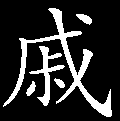
\includegraphics[width=3mm]{../Images/00005}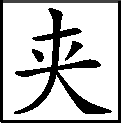
\includegraphics[width=3mm]{../Images/00012}\footnotesize \kaishu 必有是语,方是黛玉。此又系黛玉平生之病。}宝玉笑而不答。{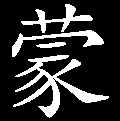
\includegraphics[width=3mm]{../Images/00006}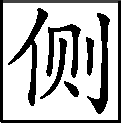
\includegraphics[width=3mm]{../Images/00011}\footnotesize \kaishu 黛玉之问,宝玉之笑,两心一照,何等神工鬼斧文章。}一径同秦钟上学去了。

原来这贾家义学离此也不甚远,不过一里之遥,原系当日始祖所立,恐族中子弟有贫穷不能请师者,即入此中肄业。凡族中有官爵之人,皆供给银两,按俸之多寡帮助,为学中之费。特共举年高有德之人为塾掌,专为训课子弟。{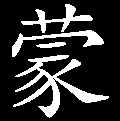
\includegraphics[width=3mm]{../Images/00006}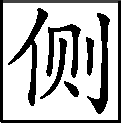
\includegraphics[width=3mm]{../Images/00011}\footnotesize \kaishu 创立者之用心,可谓至矣。}如今宝秦二人来了,一一的都互相拜见过,读起书来。自此以后,他二人同来同往,同起同坐,愈加亲密。又兼贾母爱惜,也时常的留下秦钟,住上三天五日,与自己的重孙一般疼爱。因见秦钟不甚宽裕,更又助他些衣履等物。不上一月之工,秦钟在荣府便熟了。{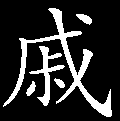
\includegraphics[width=3mm]{../Images/00005}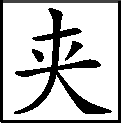
\includegraphics[width=3mm]{../Images/00012}\footnotesize \kaishu 交待的清。}宝玉终是不安分之人,{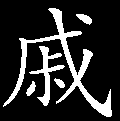
\includegraphics[width=3mm]{../Images/00005}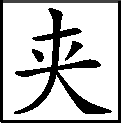
\includegraphics[width=3mm]{../Images/00012}\footnotesize \kaishu 写宝玉总作如此笔。}竟一味的随心所欲,因此又发了癖性,又特向秦钟悄说道:``咱们两个人一样的年纪,况又是同窗,以后不必论叔侄,只论弟兄朋友就是了。''{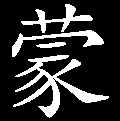
\includegraphics[width=3mm]{../Images/00006}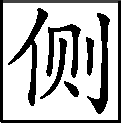
\includegraphics[width=3mm]{../Images/00011}\footnotesize \kaishu 悄说之时何时?舍尊就卑何心?随心所欲何癖?相亲爱密何情?}先是秦钟不肯,当不得宝玉不依,只叫他``兄弟'',或叫他的表字``鲸卿'',秦钟也只得混着乱叫起来。

原来这学中虽都是本族人丁与些亲戚家的子弟,俗语说的好,``一龙生九种,九种各别。''未免人多了,就有龙蛇混杂,下流人物在内。{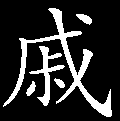
\includegraphics[width=3mm]{../Images/00005}\includegraphics[width=3mm]{../Images/00012}\footnotesize \kaishu 伏一笔。}自宝、秦二人来了,都生的花朵儿一般的模样,又见秦钟腼腆温柔,未语面先红,怯怯羞羞,有女儿之风;宝玉又是天生成惯能做小服低,赔身下气,性情体贴,话语绵缠,{\includegraphics[width=3mm]{../Images/00005}\includegraphics[width=3mm]{../Images/00012}\footnotesize \kaishu 凡四语十六字,上用``天生成''三字,真正写尽古今情种人也。}因此二人更加亲厚,也怨不得那起同窗人起了疑,背地里你言我语,诟谇谣诼,布满书房内外。{\includegraphics[width=3mm]{../Images/00005}\includegraphics[width=3mm]{../Images/00012}\footnotesize \kaishu 伏下文``阿呆争风''一回。}

原来薛蟠自来王夫人处住后,便知有一家学,学中广有青年子弟,不免偶动了龙阳之兴,因此也假来上学读书,不过是三日打鱼,两日晒网,白送些束修礼物与贾代儒,却不曾有一些儿进益,只图结交些契弟。谁想这学内就有好几个小学生,图了薛蟠的银钱吃穿,被他哄上手的,也不消多记。{\includegraphics[width=3mm]{../Images/00005}\includegraphics[width=3mm]{../Images/00012}\footnotesize \kaishu 先虚写几个淫浪蠢物,以陪下文,方不孤不板。 \includegraphics[width=3mm]{../Images/00009}\includegraphics[width=3mm]{../Images/00012}\footnotesize \kaishu 伏下金荣。}更有两个多情的小学生,{\includegraphics[width=3mm]{../Images/00005}\includegraphics[width=3mm]{../Images/00012}\footnotesize \kaishu 此处用``多情''二字方妙。}亦不知是那一房的亲眷,亦未考真名姓,{\includegraphics[width=3mm]{../Images/00005}\includegraphics[width=3mm]{../Images/00012}\footnotesize \kaishu 一并隐其姓名,所谓``具菩提之心,秉刀斧之笔''。}只因生得妩媚风流,满学中都送了他两个外号,一号``香怜'',一号``玉爱''。谁都有窃慕之意,将不利于孺子之心,{\includegraphics[width=3mm]{../Images/00005}\includegraphics[width=3mm]{../Images/00012}\footnotesize \kaishu 诙谐得妙,又似李笠翁书中之趣语。}只是都惧薛蟠的威势,不敢来沾惹。如今宝、秦二人一来了,见了他两个,也不免缱绻羡爱,亦因知系薛蟠相知,故未敢轻举妄动。香、玉二人心中,也一般的留情与宝、秦。因此四人心中虽有情意,只未发迹。每日一入学中,四处各坐,却八目勾留,或设言托意,或咏桑寓柳,遥以心照,却外面自为避人眼目。{\includegraphics[width=3mm]{../Images/00005}\includegraphics[width=3mm]{../Images/00012}\footnotesize \kaishu 小儿之态活现,掩耳偷铃者亦然,世人亦复不少。}不意偏又有几个滑贼看出形景来,都背后挤眉弄眼,或咳嗽扬声,{\includegraphics[width=3mm]{../Images/00005}\includegraphics[width=3mm]{../Images/00012}\footnotesize \kaishu 又画出历来学中一群顽皮来。 \includegraphics[width=3mm]{../Images/00006}\includegraphics[width=3mm]{../Images/00011}\footnotesize \kaishu 才子辈偏无不解之事。}这也非此一日。

可巧这日代儒有事,早已回家去了,又留下一句七言对联,命学生对了,明日再来上书;将学中之事,又命贾瑞{\includegraphics[width=3mm]{../Images/00005}\includegraphics[width=3mm]{../Images/00012}\footnotesize \kaishu 又出一贾瑞。}暂且管理。妙在薛蟠如今不大来学中应卯了,因此秦钟趁此和香怜挤眉弄眼,递暗号儿,二人假装出小恭,走至后院说体己话。秦钟先问他:``家里的大人可管你交朋友不管?''{\includegraphics[width=3mm]{../Images/00005}\includegraphics[width=3mm]{../Images/00012}\footnotesize \kaishu 妙问,真真活跳出两个小儿来。}一语未了,只听背后咳嗽了一声。{\includegraphics[width=3mm]{../Images/00005}\includegraphics[width=3mm]{../Images/00012}\footnotesize \kaishu 太急了些,该再听他二人如何结局,正所谓小儿之态也,酷肖之极。}二人唬的忙回头看时,原来是窗友名金荣{\includegraphics[width=3mm]{../Images/00005}\includegraphics[width=3mm]{../Images/00012}\footnotesize \kaishu 妙名,盖云有金自荣,廉耻何益哉?}者。香怜本有些性急,羞怒相激,问他道:``你咳嗽什么?难道不许我两个说话不成?''金荣笑道:``许你们说话,难道不许我咳嗽不成?我只问你们:有话不明说,许你们这样鬼鬼祟祟的干什么故事?我可也拿住了,还赖什么!先得让我抽个头儿,咱们一声儿不言语,不然大家就奋起来。''秦、香二人急得飞红的脸,便问道:``你拿住什么了?''金荣笑道:``我现拿住了是真的。''说着,又拍着手笑嚷道:``贴的好烧饼!你们都不买一个吃去?''秦钟、香怜二人又气又急,忙进来向贾瑞前告金荣,说金荣无故欺负他两个。

原来这贾瑞最是个图便宜没行止的人,每在学中以公报私,勒索子弟们请他;{\includegraphics[width=3mm]{../Images/00006}\includegraphics[width=3mm]{../Images/00011}\footnotesize \kaishu 学中亦自有此辈,可为痛哭。}后又附助着薛蟠,图些银钱酒肉,一任薛蟠横行霸道,他不但不去管约,反助纣为虐讨好儿。偏那薛蟠本是浮萍心性,今日爱东,明日爱西,近来又有了新朋友,把香、玉二人丢开一边。就连金荣亦是当日的好朋友,自有了香、玉二人,便弃了金荣。近日连香、玉亦已见弃。故贾瑞也无了提携帮衬之人,不说薛蟠得新弃旧,只怨香、玉二人不在薛蟠前提携帮补他,{\includegraphics[width=3mm]{../Images/00005}\includegraphics[width=3mm]{../Images/00012}\footnotesize \kaishu 无耻小人,真有此心。}因此贾瑞金荣等一干人,也正在醋妒他两个。今儿见秦、香二人来告金荣,贾瑞心中便不自在起来,不好呵叱秦钟,却拿着香怜作法,反说他多事,着实抢白了几句。香怜反讨了没趣,连秦钟也讪讪的各归坐位去了。金荣越发得了意,摇头咂嘴的,口内还说许多闲话,玉爱偏又听了不忿,两个人隔座咕咕唧唧的角起口来。金荣只一口咬定说:``方才明明的撞见他两个在后院子里亲嘴摸屁股,两个商议定了,一对一肏,撅草棍儿抽长短,{\includegraphics[width=3mm]{../Images/00006}\includegraphics[width=3mm]{../Images/00011}\footnotesize \kaishu ``怎么长短''四字,何等韵雅,何等浑含!俚语得文人提来,便觉有金玉为声之象。}\href{../Text/part0013_split_000.html\#lnkback_1_a}{\textsuperscript{①}}谁长谁先干。''金荣只顾得意乱说,却不防还有别人。谁知早又触怒了一个。你道这个是谁?

原来这一个名唤贾蔷,{\includegraphics[width=3mm]{../Images/00005}\includegraphics[width=3mm]{../Images/00012}\footnotesize \kaishu 新而艳,得空便入。}亦系宁府中之正派玄孙,父母早亡,从小儿跟贾珍过活,如今长了十六岁,比贾蓉生的还风流俊俏。他兄弟二人最相亲厚,常相共处。宁府人多口杂,那些不得志的奴仆们,专能造言诽谤主人,因此不知又有了什么小人诟谇谣诼之辞。贾珍想亦风闻得些口声不大好,自己也要避些嫌疑,如今竟分与房舍,命贾蔷搬出宁府,自去立门户过活去了。{\includegraphics[width=3mm]{../Images/00006}\includegraphics[width=3mm]{../Images/00011}\footnotesize \kaishu 此等嫌疑不敢认真搜查,悄为分计,皆以含而不露为文,真是灵活至极之笔。}这贾蔷外相既美,{\includegraphics[width=3mm]{../Images/00005}\includegraphics[width=3mm]{../Images/00012}\footnotesize \kaishu 亦不免招谤,难怪小人之口。}内性又聪明,虽然应名来上学,亦不过虚掩眼目而已。仍是斗鸡走狗,赏花玩柳。总恃上有贾珍溺爱,{\includegraphics[width=3mm]{../Images/00005}\includegraphics[width=3mm]{../Images/00012}\footnotesize \kaishu 贬贾珍最重。}下有贾蓉匡助,{\includegraphics[width=3mm]{../Images/00005}\includegraphics[width=3mm]{../Images/00012}\footnotesize \kaishu 贬贾蓉次之。}因此族中人谁敢来触逆于他。他既和贾蓉最好,今见有人欺负秦钟,如何肯依?如今自己要挺身出来报不平,心中却忖度一番,{\includegraphics[width=3mm]{../Images/00005}\includegraphics[width=3mm]{../Images/00012}\footnotesize \kaishu 这一忖度,方是聪明人之心机,写得最好看,最细致。}想道:``金荣贾瑞一干人,都是薛大叔的相知,向日我又与薛大叔相好,倘或我一出头,他们告诉了老薛,{\includegraphics[width=3mm]{../Images/00005}\includegraphics[width=3mm]{../Images/00012}\footnotesize \kaishu 先曰``薛大叔'',次曰``老薛'',写尽骄侈纨绔。}我们岂不伤和气?待要不管,如此谣言,说的大家没趣。如今何不用计制服,又止息了口声,又不伤了脸面。''想毕,也装出小恭,走至外面,悄悄的把跟宝玉的书童名唤茗烟{\includegraphics[width=3mm]{../Images/00005}\includegraphics[width=3mm]{../Images/00012}\footnotesize \kaishu 又出一茗烟。}者唤到身边,如此这般调拨他几句。{\includegraphics[width=3mm]{../Images/00005}\includegraphics[width=3mm]{../Images/00012}\footnotesize \kaishu 如此便好,不必细述。}

这茗烟乃是宝玉第一个得用的,且又年轻不谙世事,如今听贾蔷说金荣如此欺负秦钟,连他爷宝玉都干连在内,不给他个利害,下次越发狂纵难制了。这茗烟无故就要欺压人的,如今得了这个信,又有贾蔷助着,便一头进来找金荣,也不叫金相公了,只说:``姓金的,你是什么东西!''贾蔷遂跺一跺靴子,故意整整衣服,看看日影儿说:``是时候了。''遂先向贾瑞说有事要早一步。贾瑞不敢强他,只得随他去了。这里茗烟先一把揪住金荣,{\includegraphics[width=3mm]{../Images/00006}\includegraphics[width=3mm]{../Images/00011}\footnotesize \kaishu 豪奴辈,虽系主人亲故亦随便欺慢,即有一二不服气者,而豪家多是偏护家人。理之所无,而事之尽有,不知是何心思,实非凡常可能测略。}问道:``我们肏屁股不肏屁股,管你\includegraphics[width=8mm]{../images/00022}相干?横竖没肏你爹去罢了!你是好小子,出来动一动你茗大爷!''吓的满屋中子弟都怔怔的痴望。贾瑞忙吆喝:``茗烟不得撒野!''金荣气黄了脸,说:``反了!奴才小子都敢如此,我和你主子说。''便夺手要去抓打宝玉秦钟。{\includegraphics[width=3mm]{../Images/00005}\includegraphics[width=3mm]{../Images/00012}\footnotesize \kaishu 好看之极!}尚未去时,从脑后``飕''的一声,早见一方砚瓦飞来,{\includegraphics[width=3mm]{../Images/00005}\includegraphics[width=3mm]{../Images/00012}\footnotesize \kaishu 好看好笑之极!}并不知系何人打来的,幸未打着,却又打了旁人的座上,这座上乃是贾兰、贾菌。

贾菌亦系荣府近派的重孙,{\includegraphics[width=3mm]{../Images/00005}\includegraphics[width=3mm]{../Images/00012}\footnotesize \kaishu 先写一宁派,又写一荣派,互相错综得妙。}其母亦少寡,独守着贾菌,这贾菌与贾兰最好,所以二人同桌而坐。谁知贾菌年纪虽小,志气最大,极是淘气不怕人的。{\includegraphics[width=3mm]{../Images/00005}\includegraphics[width=3mm]{../Images/00012}\footnotesize \kaishu 要知没志气小儿,必不会淘气。}他在座上冷眼看见金荣的朋友暗助金荣,飞砚来打茗烟,偏没打着茗烟,便落在他座上,正打在面前,将一个磁砚水壶打了个粉碎,溅了一书黑水。{\includegraphics[width=3mm]{../Images/00005}\includegraphics[width=3mm]{../Images/00012}\footnotesize \kaishu 这等忙,有此闲处用笔。}贾菌如何依得,便骂:``好囚攮的们,这不都动了手了么!''{\includegraphics[width=3mm]{../Images/00005}\includegraphics[width=3mm]{../Images/00012}\footnotesize \kaishu 好听煞。}骂着,也抓起砚砖来要飞。{\includegraphics[width=3mm]{../Images/00005}\includegraphics[width=3mm]{../Images/00012}\footnotesize \kaishu 先瓦砚,次砖砚,转换得妙极。}贾兰是个省事的,忙按住砚,极口劝道:``好兄弟,不与咱们相干。''{\includegraphics[width=3mm]{../Images/00005}\includegraphics[width=3mm]{../Images/00012}\footnotesize \kaishu 是贾兰口气。}贾菌如何忍得住,便两手抱起书匣子来,照那边抡了去。{\includegraphics[width=3mm]{../Images/00005}\includegraphics[width=3mm]{../Images/00012}\footnotesize \kaishu 先``飞''后``抡'',用字得神,好看之极!}终是身小力薄,却抡不到那里,刚到宝玉秦钟桌案上就落了下来,只听``哗啷啷''一声,砸在桌上,书本纸片等至于笔砚之物撒了一桌,又把宝玉的一碗茶也砸得碗碎茶流。{\includegraphics[width=3mm]{../Images/00005}\includegraphics[width=3mm]{../Images/00012}\footnotesize \kaishu 好看之极!不打着别个,偏打着二人,亦想不到文章也。此书此等笔法,与后文踢着袭人、误打平儿,是一样章法。}贾菌便跳出来,要揪打那一个飞砚的。金荣此时随手抓了一根毛竹大板在手,地狭人多,那里经得舞动长板。茗烟早吃了一下,乱嚷:``你们还不来动手!''宝玉还有三个小厮:一名锄药,一名扫红,一名墨雨。这三个岂有不淘气的,一齐乱嚷:``小妇养的!动了兵器了!''{\includegraphics[width=3mm]{../Images/00005}\includegraphics[width=3mm]{../Images/00012}\footnotesize \kaishu 好听之极,好看之极!}墨雨遂掇起一根门闩,扫红锄药手中都是马鞭子,蜂拥而上。贾瑞急拦一回这个,劝一回那个,谁听他的话,肆行大闹。众顽童也有趁势帮着打太平拳助乐的,也有胆小藏在一边的,也有直立在桌上拍着手儿乱笑、喝着声儿叫打的,登时间鼎沸起来。{\includegraphics[width=3mm]{../Images/00006}\includegraphics[width=3mm]{../Images/00011}\footnotesize \kaishu 燕青打擂台,也不过如此。}

外边李贵等几个大仆人听见里边作反起来,忙都进来一齐喝住。问是何原故。众声不一,这一个如此说,那一个又如彼说。{\includegraphics[width=3mm]{../Images/00005}\includegraphics[width=3mm]{../Images/00012}\footnotesize \kaishu 妙!如闻其声。}李贵且喝骂了茗烟四个一顿,{\includegraphics[width=3mm]{../Images/00005}\includegraphics[width=3mm]{../Images/00012}\footnotesize \kaishu 处治的好。}撵了出去。秦钟的头早撞在金荣的板上,打去一层油皮,宝玉正拿褂襟子替他揉呢,见喝住了众人,便命:``李贵,收书!拉马来,我回去回太爷去!我们被人欺负了,不敢说别的,守礼来告诉瑞大爷,瑞大爷反倒派我们不是,听人家骂我们,还调唆他们打我们。茗烟见人欺负我,他岂有不为我的;他们反打伙儿打了茗烟,连秦钟的头也打破了,还在这里念什么书!不如散了罢。''李贵劝道:``哥儿不要性急。太爷既有事回家去了,这会子为这点子事去聒噪他老人家,倒显的咱们没理。依我的主意,那里的事那里了结好,何必去惊动他老人家。这都是瑞大爷的不是,太爷不在这里,你老人家就是这学里的头脑了,众人看你行事。{\includegraphics[width=3mm]{../Images/00006}\includegraphics[width=3mm]{../Images/00011}\footnotesize \kaishu 劝的心思,有个太爷得知,未必然之。故巧为辗转以结其局,而不失其体。}众人有了不是,该打的打,该罚的罚,如何等闹到这步田地不管?''贾瑞道:``我吆喝着都不听。''{\includegraphics[width=3mm]{../Images/00005}\includegraphics[width=3mm]{../Images/00012}\footnotesize \kaishu 如闻。}李贵笑道:``不怕你老人家恼我,素日你老人家到底有些不正经,所以这些兄弟才不听。就闹到太爷跟前去,连你老人家也脱不过的。还不快作主意撕罗开了罢。''宝玉道:``撕罗什么?我必是回去的!''秦钟哭道:``有金荣,我是不在这里念书的。''宝玉道:``这是为什么?难道有人家来得的,咱们倒来不得?我必回明白众人,撵了金荣去。''又问李贵:``金荣是那一房的亲戚?''李贵想了一想:``也不用问了。若说起那一房的亲戚,更伤了弟兄们的和气了。''

茗烟在窗外道:``他是东胡同里璜大奶奶的侄儿,那是什么硬正仗腰子的,也来唬我们。璜大奶奶是他姑娘。你那姑妈只会打旋磨儿,给我们琏二奶奶跪着借当头。{\includegraphics[width=3mm]{../Images/00006}\includegraphics[width=3mm]{../Images/00011}\footnotesize \kaishu 可怜!开口告人,终身是玷。}我眼里就看不起他那样的主子奶奶!''李贵忙断喝不止,说:``偏你这小狗肏的知道,有这些蛆嚼!''宝玉冷笑道:``我只当是谁的亲戚,原来是璜嫂子的侄儿,我就去问问他来!''说着便要走,叫茗烟进来包书。茗烟包着书,又得意道:``爷也不用自己去见,等我去到他家,就说老太太有说的话问他呢,雇上一辆车拉进去,当着老太太问他,岂不省事?''{\includegraphics[width=3mm]{../Images/00005}\includegraphics[width=3mm]{../Images/00012}\footnotesize \kaishu 又以贾母欺压,更妙!}李贵忙喝道:``你要死!仔细回去我好不好先捶了你,然后再回老爷太太,就说宝玉全是你调唆的。我这里好容易劝哄的好了一半了,你又来生个新法子。你闹了学堂,不说变法儿压息了才是,倒要往大里奋\href{../Text/part0013_split_000.html\#lnkback_2_a}{\textsuperscript{②}}!''茗烟方不敢作声儿了。

此时贾瑞也怕闹大了,自己也不干净,只得委曲着来央告秦钟,又央告宝玉。先是他二人不肯。后来宝玉说:``不回去也罢了,只叫金荣赔不是便罢。''金荣先是不肯,后来禁不得贾瑞也来逼他去赔不是,李贵等只得好劝金荣说:``原来是你起的端,你不这样,怎得了局?''金荣强不得,只得与秦钟作了揖。宝玉还不依,偏定要磕头。

贾瑞只要暂息此事,又悄悄的劝金荣说:``俗语说得好:`杀人不过头点地。'你既惹出事来,少不得下点气儿,磕个头就完事了。''金荣无奈,只得进前来与秦钟磕头。且听下回分解。\href{../Text/part0013_split_000.html\#lnkback_3_a}{\textsuperscript{③}}

{\includegraphics[width=3mm]{../Images/00005}\kaishu 总评:此篇写贾氏学中,非亲即族,且学乃大众之规范,人伦之根本。首先悖乱,以至于此极,其贾家之气数,即此可知。挟用袭人之风流,群小之恶逆,一扬一抑,作者自必有所取。}

%{\href{../Text/part0013_split_000.html\#navto_1_a}{①}按:蒙、戚本正文金荣的话删去了脏字,作``方才明明的撞见他两个在后院里商议着什么长短。''以金荣的性格说话不当这么含蓄。此系版本时有这种修改文字后自称自赞的情况。}
%
%{\href{../Text/part0013_split_000.html\#navto_2_a}{②}此语各本异文较多,列本作``往大里奋'',己、庚、杨本同作``往大里闹'',戚、蒙本作``迈火坑'',甲辰本作``往火里奋'',舒本作``往火里奔'',而程甲本则作``往火里奔查''。从这些异文看,原文当是``往大里奋'',而在传抄过程中,分化成两种情况:一种是己、庚、杨本一系因疑``奋''字不通而改为``闹''字。另一种先是``大''字形讹为``火''字(如甲辰本),因``奋''字费解而校改为音、形兼近的``奔''字(如舒本、程甲本。程甲本的``奔查''校改痕迹明显:``查''字当系被点改的``奋''字的误认加重抄);戚、蒙本改动更随意,仅保留了``火''字。``往大里奋''的``奋''字,可能是方言,准确意思未详。但其本义就有振作、鼓气之意,用在此处也还可解。前文金荣有``不然大家就奋起来''一语,可与此处互证。}
%
%{\href{../Text/part0013_split_000.html\#navto_3_a}{③}此回结尾文字各本存在较大差异,笔者认为舒本文字更接近原貌(参见附录``校读札记'')。但为了与下回衔接,此处暂依戚本。}
